\documentclass{article}
\usepackage{xcolor}
\usepackage{tikz}
\usepackage{pgfplots}
\usepackage{pgf-pie}

\definecolor{vermelho}{HTML}{D7191C}
\definecolor{laranja}{HTML}{FD9B61}
\definecolor{verde}{HTML}{91C3AB}
\definecolor{azul}{HTML}{2B83BA}
\definecolor{violeta}{HTML}{AC146D}
\definecolor{amarelo}{HTML}{D2D221}

\errorcontextlines 10000

\begin{document}

%TODO Macro não funciona
%\newcommand{barchart}[4]{
%	\begin{figure}[h]\centering
%	\begin{tikzpicture}\begin{axis}[
%		ybar stacked,
%		legend style={
%		    legend columns=#2
%		    at={(xticklabel cs:0.5)},
%		    anchor=north,
%		    draw=none
%		},
%		xtick=data,
%		width=0.7\textwidth,
%%	    symbolic x coords={?,1974 -- 1978,1979 -- 1983,1984 -- 1988,1989 -- 1993,1994 -- 1998,1999 -- 2003,2004 -- 2008,2009 -- 2013},
%		x tick label style={rotate=45,anchor=east},
%	]
%	#1
%	\legend{#3}
%	\end{axis}\end{tikzpicture}
%	\caption{#4}
%	\end{figure}
%}


%\barchart{
%	\addplot[vermelho,fill=vermelho] coordinates { (1,3) (2,1) (3,1) (4,1) (5,1) (6,3) (7,1) (8,1) };
%	\addplot[laranja,fill=laranja] coordinates { (1,3) (2,1) (3,1) (4,1) (5,1) (6,3) (7,1) (8,1) };
%	\addplot[amarelo,fill=amarelo] coordinates { (1,3) (2,5) (3,7) (4,8) (5,3) (6,5) (7,7) (8,8) };
%	\addplot[verde,fill=verde] coordinates { (1,2) (2,2) (3,1) (4,1) (5,2) (6,2) (7,1) (8,1) };
%	\addplot[azul,fill=azul] coordinates { (1,3) (2,1) (3,1) (4,1) (5,1) (6,3) (7,1) (8,1) };
%	\addplot[violeta,fill=violeta] coordinates { (1,3) (2,1) (3,1) (4,1) (5,1) (6,3) (7,1) (8,1) };
%}{6}{Vermelho,Laranja,Amarelo,Verde,Azul,Violeta}{Lorem ipsum dolor sit amet}


\begin{figure}[h]\centering
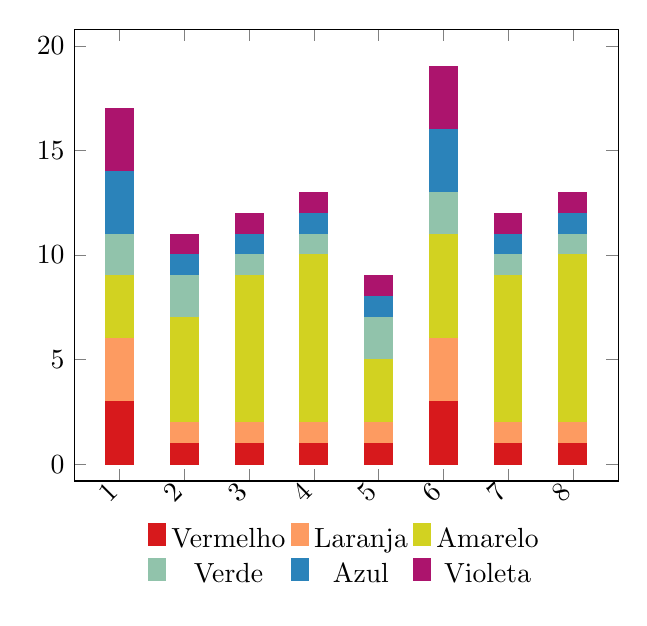
\begin{tikzpicture}\begin{axis}[
    ybar stacked,
    legend style={
        legend columns=3,
        at={(xticklabel cs:0.5)},
        anchor=north,
        draw=none
    },
    xtick=data,
    width=0.7\textwidth,
%    symbolic x coords={?,1974 -- 1978,1979 -- 1983,1984 -- 1988,1989 -- 1993,1994 -- 1998,1999 -- 2003,2004 -- 2008,2009 -- 2013},
	x tick label style={rotate=45,anchor=east},
]
\addplot[vermelho,fill=vermelho] coordinates { (1,3) (2,1) (3,1) (4,1) (5,1) (6,3) (7,1) (8,1) };
\addplot[laranja,fill=laranja] coordinates { (1,3) (2,1) (3,1) (4,1) (5,1) (6,3) (7,1) (8,1) };
\addplot[amarelo,fill=amarelo] coordinates { (1,3) (2,5) (3,7) (4,8) (5,3) (6,5) (7,7) (8,8) };
\addplot[verde,fill=verde] coordinates { (1,2) (2,2) (3,1) (4,1) (5,2) (6,2) (7,1) (8,1) };
\addplot[azul,fill=azul] coordinates { (1,3) (2,1) (3,1) (4,1) (5,1) (6,3) (7,1) (8,1) };
\addplot[violeta,fill=violeta] coordinates { (1,3) (2,1) (3,1) (4,1) (5,1) (6,3) (7,1) (8,1) };
\legend{Vermelho,Laranja,Amarelo,Verde,Azul,Violeta}
\end{axis}\end{tikzpicture}
\caption{Lorem ipsum}
\end{figure}

\begin{figure}[h]\centering
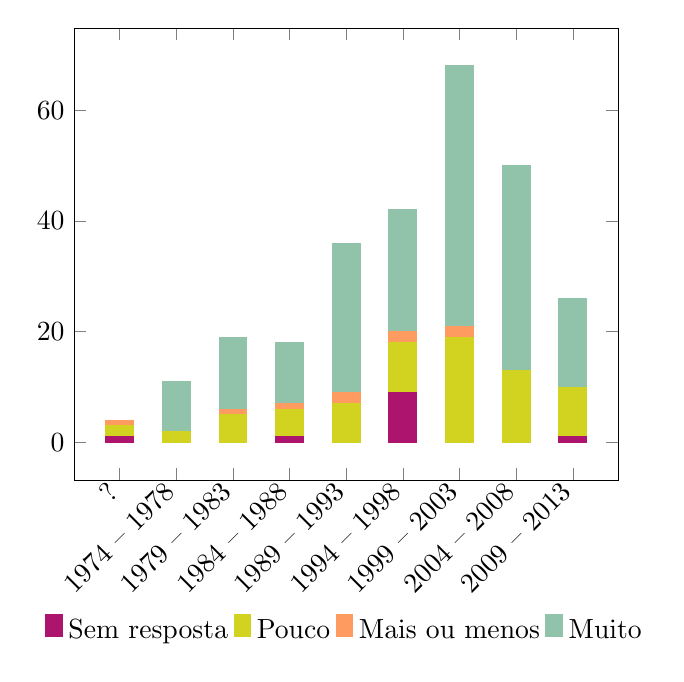
\begin{tikzpicture}\begin{axis}[
    ybar stacked,
    legend style={
        legend columns=4,
        at={(xticklabel cs:0.5)},
        anchor=north,
        draw=none
    },
    xtick=data,
    width=0.7\textwidth,
    symbolic x coords={?,1974 -- 1978,1979 -- 1983,1984 -- 1988,1989 -- 1993,1994 -- 1998,1999 -- 2003,2004 -- 2008,2009 -- 2013},
	x tick label style={rotate=45,anchor=east},
]
\addplot[violeta,fill=violeta] coordinates { (?, 1) (1974 -- 1978, 0) (1979 -- 1983, 0)  (1984 -- 1988, 1)  (1989 -- 1993, 0)  (1994 -- 1998, 9)  (1999 -- 2003, 0 ) (2004 -- 2008, 0)  (2009 -- 2013, 1) };
\addplot[amarelo,fill=amarelo] coordinates { (?, 2) (1974 -- 1978, 2) (1979 -- 1983, 5)  (1984 -- 1988, 5)  (1989 -- 1993, 7)  (1994 -- 1998, 9)  (1999 -- 2003, 19) (2004 -- 2008, 13) (2009 -- 2013, 9) };
\addplot[laranja,fill=laranja] coordinates { (?, 1) (1974 -- 1978, 0) (1979 -- 1983, 1)  (1984 -- 1988, 1)  (1989 -- 1993, 2)  (1994 -- 1998, 2)  (1999 -- 2003, 2)  (2004 -- 2008, 0)  (2009 -- 2013, 0)};
    \addplot[verde,fill=verde] coordinates { (?, 0) (1974 -- 1978, 9) (1979 -- 1983, 13) (1984 -- 1988, 11) (1989 -- 1993, 27) (1994 -- 1998, 22) (1999 -- 2003, 47) (2004 -- 2008, 37) (2009 -- 2013, 16) };
\legend{Sem resposta,Pouco,Mais ou menos,Muito}
\end{axis}\end{tikzpicture}
\caption{Você considera o BCC foi importante para a sua formação profissional?}
\end{figure}



\end{document}
